\documentclass[17pt]{article}
\usepackage[utf8]{inputenc}
\usepackage{amsmath}
\usepackage{graphicx}
\usepackage{hyperref}
\usepackage{listings}
\usepackage{color}
\hypersetup{
    colorlinks=true,
    linkcolor=blue,
    filecolor=magenta,      
    urlcolor=cyan,
}
 
\urlstyle{same}
\definecolor{codegreen}{rgb}{0,0.6,0}
\definecolor{codegray}{rgb}{0.5,0.5,0.5}
\definecolor{codepurple}{rgb}{0.58,0,0.82}
\definecolor{backcolour}{rgb}{0.95,0.95,0.92}
\lstdefinestyle{mystyle}{
    backgroundcolor=\color{backcolour},   
    commentstyle=\color{codegreen},
    keywordstyle=\color{magenta},
    numberstyle=\tiny\color{codegray},
    stringstyle=\color{codepurple},
    basicstyle=\footnotesize,
    breakatwhitespace=false,         
    breaklines=true,                 
    captionpos=b,                    
    keepspaces=true,                 
    numbers=left,                    
    numbersep=5pt,                  
    showspaces=false,                
    showstringspaces=false,
    showtabs=false,                  
    tabsize=2
}
\lstset{style=mystyle}
\graphicspath{ {../Plots/} }
\title{
	{\large Statistical learning: 4th assignment}\\}
\author{Ali Zamani(96123035) \& Aryan Nasehzadeh}
\begin{document}
\maketitle

\newpage
\section{Machin leraning algorithms}
In this section, we will use different machine learning algorithms such as LDA, QDA, KNN, Decision tree, and kernel SVM. To access source code you can check the link:\\
The sklearn package is used.
Dataset has numbers of unknown features, one way is dropping all data with the unknown feature but in this approach, we lose a lot of data thus we should use other approaches. 
We replace unknown features with mean or min or max of features on that class, for example, if the unknown feature is associated with data in class 1, we replace that feature with the mean of features on class 1. we also train our model with scaled and unscaled data and results are reported in tables \ref{QDATable}, \ref{LDAtable}, \ref{treeTable} , \ref{KNNTable} , \ref{SVMTable}. In the SVM algorithm non-scaled data are used. As you see maximum accuracy belongs to \textbf{polynomial kernel SVM} and it is \textbf{58\%}.
\section{Neural Network(NN)}
In this section, we will create an NN model with 3 hidden layers. We use shuffled and unscaled data. Table \ref{NN} shows results for different neurons numbers in each layer. Figure \ref{figNN} show another result. As you can see in table \ref{NN} maximum test accuracy is 28\% and it is less than 58\% thus kernel SVM with polynomial kernel has better test accuracy.
\newpage
% QDA table
\begin{table}[]
	\caption{QDA}
	\centering
	\label{QDATable}
	\begin{tabular}{|l|l|l|l|}
		\hline
		\multicolumn{4}{|c|}{QDA}\\
		\cline{1-4}
		\hline
		Train & Merged & Scaled & ACC \\
		\cline{2-4}
		 &    Yes      &   Yes    & 75\%  \\
		\cline{2-4}
		&    Yes      &   No     & 92\%\\
		\cline{2-4}
		& No & Yes &  54\%\\
		\cline{2-4}
		& No & No & 96\%\\
		\hline
		
		Test & Yes & Yes & 5.2\% \\
		\cline{2-4}
		&    Yes      &   No     & 27\%\\
		\cline{2-4}
		& No & Yes & 0\% \\
		\cline{2-4}
		& No & No & 23\%\\
		\hline
	\end{tabular}
\end{table}

% LDA table
\begin{table}[]
	\caption{LDA}
	\label{LDAtable}
	\centering
	\begin{tabular}{|l|l|l|l|}
		\hline
		\multicolumn{4}{|c|}{LDA}\\
		\cline{1-4}
		\hline
		Train & Merged & Scaled & ACC \\
		\cline{2-4}
		&    Yes      &   Yes    & 75\%  \\
		\cline{2-4}
		&    Yes      &   No     & 92\% \\
		\cline{2-4}
		& No & Yes & 54\% \\
		\cline{2-4}
		& No & No & 96\%\\
		\hline
		
		Test & Yes & Yes & 1\% \\
		\cline{2-4}
		&    Yes      &   No     & 27\%\\
		\cline{2-4}
		& No & Yes & 2.2\% \\
		\cline{2-4}
		& No & No & 47\%\\
		\hline
	\end{tabular}
\end{table}

% Decision tree table
\begin{table}[]
	\caption{Decision tree}
	\centering
	\label{treeTable}
	\begin{tabular}{|l|l|l|l|}
		\hline
		\multicolumn{4}{|c|}{Decision tree}\\
		\cline{1-4}
		\hline
		Train & Merged & Scaled & ACC \\
		\cline{2-4}
		&    Yes      &   Yes    & 75\%  \\
		\cline{2-4}
		&    Yes      &   No     & 92\%\\
		\cline{2-4}
		& No & Yes & 54\% \\
		\cline{2-4}
		& No & No & 96\%\\
		\hline
		
		Test & Yes & Yes & 11\% \\
		\cline{2-4}
		&    Yes      &   No     & 25\%\\
		\cline{2-4}
		& No & Yes & 2.6\% \\
		\cline{2-4}
		& No & No & 25\%\\
		\hline
	\end{tabular}
\end{table}

% KNN table
\begin{table}[]
	\caption{KNN}
	\centering
	\label{KNNTable}
	\begin{tabular}{|l|l|l|l|}
		\hline
		\multicolumn{4}{|c|}{KNN}\\
		\cline{1-4}
		\hline
		Train & Merged & Scaled & ACC \\
		\cline{2-4}
		&    Yes      &   Yes    & 75\%  \\
		\cline{2-4}
		&    Yes      &   No     & 92\% \\
		\cline{2-4}
		& No & Yes & 54\% \\
		\cline{2-4}
		& No & No & 96\%\\
		\hline
		
		Test & Yes & Yes & 7\% \\
		\cline{2-4}
		&    Yes      &   No     & 39\%\\
		\cline{2-4}
		& No & Yes & 1.4\% \\
		\cline{2-4}
		& No & No & 40\%\\
		\hline
	\end{tabular}
\end{table}

% Kernel SVM table
\begin{table}[]
	\caption{Kernel SVM}
	\centering
	\label{SVMTable}
	\begin{tabular}{|l|l|l|l|}
		\hline
		\multicolumn{4}{|c|}{Kernel SVM}\\
		\cline{1-4}
		\hline
		Train & Merged & Kernel & ACC \\
		\cline{2-4}
		&    No      &   linear    & 96\%  \\
		\cline{2-4}
		&    No      &   polynomial     & 96\% \\
		\cline{2-4}
     	&    No      &   rbf     & 96\%\\
        \cline{2-4}
		&    No      &   sigmoid     & 96\%\\
		\cline{2-4}
		&    Yes      &   linear    & 92\%  \\
		\cline{2-4}
		&    Yes      &   polynomial     & 92\% \\
		\cline{2-4}
		&    Yes      &   rbf     & 92\%\\
		\cline{2-4}
		&    Yes      &   sigmoid     & 92\%\\
		\hline
		Test &    No      &   linear    & 51\%  \\
		\cline{2-4}
		&    No      &   polynomial     & 58\% \\
		\cline{2-4}
		&    No      &   rbf     & 4\%\\
		\cline{2-4}
		&    No      &   sigmoid     & 0.2\%\\
         \cline{2-4}
         &    Yes      &   linear    & 28\%  \\
        \cline{2-4}
        &    Yes      &   polynomial     & 25\% \\
        \cline{2-4}
        &    Yes      &   rbf     & 4\%\\
        \cline{2-4}
        &    Yes      &   sigmoid     & 0.2\%\\
		\hline
	\end{tabular}
\end{table}
\begin{table}
	\centering
	\caption{Neural Network}
	\label{NN}
	\begin{tabular}{|l|l|l|l|l|l|l|}
		\hline
		\multicolumn{7}{|c|}{Neural Network (3 layers)}\\
		\hline
		Hidden 1 & Hidden 2 & Hidden 3 & Batch size & Learning rate & Train ACC & Test ACC\\
		\hline
		40 & 30 & 20 & 40 & 0.001 & 82\% & 28\%\\
		\hline
		50 & 40 & 30 & 40 & 0.001 & 88\% & 26\%\\
		\hline
		50 & 40 & 10 & 40 & 0.001 & 79\% & 26\%\\
		\hline
		40 & 40 & 30 & 20 & 0.001 & 90\% & 24\%\\
		\hline
		200 & 150 & 100 & 40 & 0.001 & 97\% & 26\%\\
		\hline
		100 & 90 & 80 & 60 & 0.0001 & 97\% & 28\%\\
		\hline
	\end{tabular}
\end{table}
\begin{figure}
	\label{figNN}
	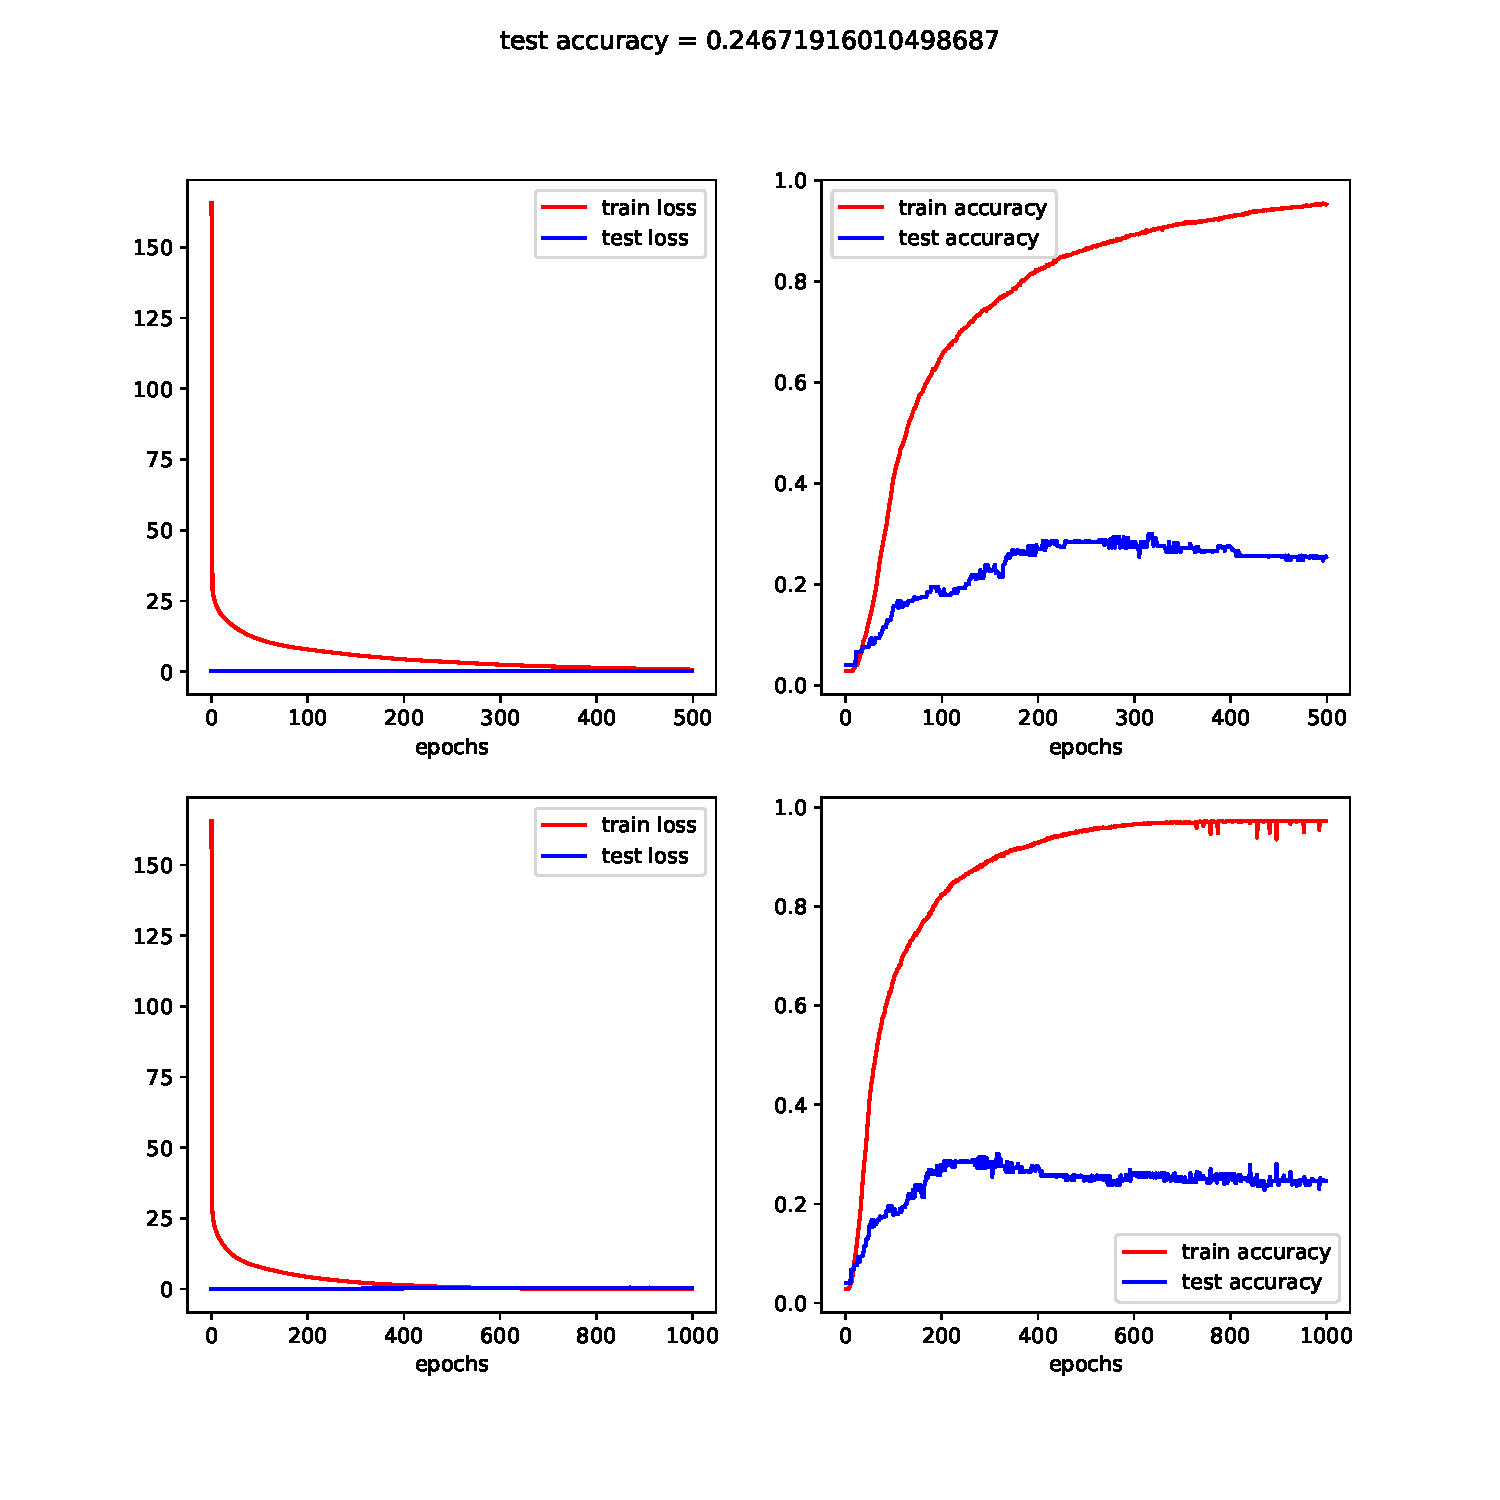
\includegraphics[scale=0.5]{results}
	\caption{Neural Network}
\end{figure}


\end{document}